\documentclass{report}

\input{~/dev/latex/template/preamble.tex}
\input{~/dev/latex/template/macros.tex}

\title{\Huge{}}
\author{\huge{Nathan Warner}}
\date{\huge{}}
\pagestyle{fancy}
\fancyhf{}
\lhead{Warner \thepage}
\rhead{}
% \lhead{\leftmark}
\cfoot{\thepage}
%\setborder
% \usepackage[default]{sourcecodepro}
% \usepackage[T1]{fontenc}

\begin{document}
    % \maketitle
        \begin{titlepage}
       \begin{center}
           \vspace*{1cm}
    
           \textbf{Calculus II} \\
           Chapter 2: Applications of Integration
    
           \vspace{0.5cm}
            
                
           \vspace{1.5cm}
    
           \textbf{Nathan Warner}
    
           \vfill
                
                
           \vspace{0.8cm}
         
           
\includegraphics[width=0.4\textwidth]{~/niu/seal.png}
                
           Computer Science \\
           Northern Illinois University\\
           September 08, 2023 \\
           United States\\
           
                
       \end{center}
    \end{titlepage}
    \tableofcontents
    \pagebreak \bigbreak \noindent
    \vspace{2in} \\
    \begin{Huge}
        \textbf{Applications \\ of Integration}
    \end{Huge}
    \bigbreak \noindent 
    \line(1,0){490}
    \bigbreak \noindent 
    \section*{\LARGE 2.1: Areas between Curves}
    \addcontentsline{toc}{section}{2.1: Areas between Curves}
    \bigbreak \noindent 
    \phantomsection
    \addcontentsline{toc}{subsection}{Area of a Region between Two Curves}
    \subsection*{Area of a Region between Two Curves}
    Let \( f(x) \) and \( g(x) \) be continuous functions over an interval \([a,b]\) such that \( f(x) \geq g(x) \) on \([a,b]\). We want to find the area between the graphs of the functions, as shown in the following figure.
    \bigbreak \noindent 
    \begin{center}
        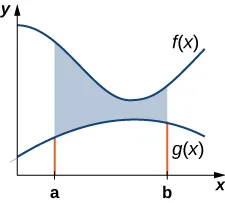
\includegraphics[scale=.5]{./figures/graph1.png  }
    \end{center}
    \bigbreak \noindent 
    As we did before, we are going to partition the interval on the \( x \)-axis
    and approximate the area between the graphs of the functions with rectangles. So, for \( i=0,1,2,\ldots,n \),
    let \( P = \{ x_i \} \)
    be a regular partition of \( [a,b] \).
    Then, for \( i=1,2,\ldots,n \),
    choose a point \( x^*_i \in [x_{i-1}, x_i] \),
    and on each interval \( [x_{i-1}, x_i] \)
    construct a rectangle that extends vertically from \( g(x^*_i) \)
    to \( f(x^*_i) \).
    Figure 2.3(a) shows the rectangles when \( x^*_i \)
    is selected to be the left endpoint of the interval and \( n=10 \).
    \begin{center}
        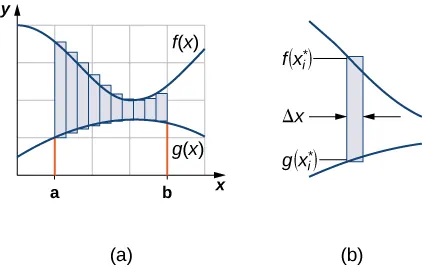
\includegraphics[scale=0.5]{ ./figures/2aaddefc-a60a-41ed-8312-ef6960ad3b6c.png }
    \end{center}
    \pagebreak \bigbreak \noindent 
    The height of each individual rectangle is \( f(x^*_i) - g(x^*_i) \) and the width of each rectangle is \( \Delta x \).
    Adding the areas of all the rectangles, we see that the area between the curves is approximated by

    \[
    A \approx \sum_{i=1}^{n} \left[ f(x^*_i) - g(x^*_i) \right] \Delta x.
    \]
    \bigbreak \noindent 
    This is a Riemann sum, so we take the limit as \( n \to \infty \) and we get
    \[
    A = \lim_{{n \to \infty}} \sum_{i=1}^{n} \left[ f(x^*_i) - g(x^*_i) \right] \Delta x = \int_{a}^{b} \left[ f(x) - g(x) \right] \, dx.
    \]
    \bigbreak \noindent 
    These findings are summarized in the following theorem.
    \bigbreak \noindent 
    \begin{thrm}[Area between two curves, integrating on the x-axis]
       Let \( f(x) \) and \( g(x) \) be continuous functions such that \( f(x) \geq g(x) \) over an interval \([a, b]\).
Let \( R \) denote the region bounded above by the graph of \( f(x) \), below by the graph of \( g(x) \), and on the left and right by the lines \( x = a \) and \( x = b \), respectively. Then, the area of \( R \) is given by

    \[
    A = \int_{a}^{b} \left[ f(x) - g(x) \right] \, dx.
    \] 
    \end{thrm}
    \bigbreak \noindent 
    Quite often, though, we want to define our interval of interest based on where the graphs of the two functions intersect. This is illustrated in the following example.
    \bigbreak \noindent 
    \begin{eg}
       If \( R \) is the region bounded above by the graph of the function \( f(x) = 9 - \left( \frac{x}{2} \right)^2 \) and below by the graph of the function \( g(x) = 6 - x \), find the area of region \( R \).
    \end{eg}
    \bigbreak \noindent \bigbreak \noindent 
    \begin{minipage}{0.47\textwidth}
    \begin{center}
        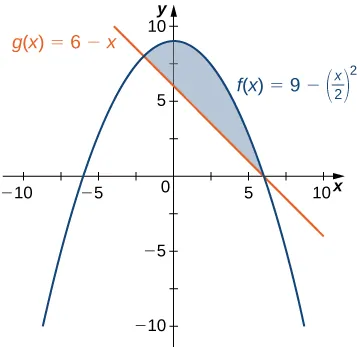
\includegraphics[scale=.35]{ ./figures/graph3.png}
    \end{center}
    \end{minipage}
    \begin{minipage}{0.47\textwidth}
        To find our limits of integration, we first need to find where the two functions intersect.
        \begin{align*}
            &=9 - \bigg(\frac{x}{2}\bigg)^{2} = 6-x \\
            &=9 - \frac{x^{2}}{4} = 6-x \\
            &=\frac{36-x^{2}}{4} = 6-x \\
            &= 36 -x^{2} = 24-4x \\
            &= -x^{2} +4x +12 \\
            &= -(x^{2}-4x-12) = 0 \\
            &= -(x-6)(x+2) \\
            &= x=6,-2
        .\end{align*}
        Thus, we need to integrate from x=-2 to 6
        \bigbreak \noindent 
    \end{minipage}
    \smallbreak \noindent
    By Theorem 1: $A = \int_{a}^{b}\ \big[f(x)-g(x)\big]\ dx $, we find that:
    \begin{align*}
        A = \frac{64}{3}\ Units^{2}
    .\end{align*}

    \pagebreak \bigbreak \noindent 
    \phantomsection
    \addcontentsline{toc}{subsection}{Areas of Compound Regions}
    \subsection*{Areas of Compound Regions}
    \bigbreak \noindent 
    So far, we have required  $f(x) \geq g(x)$ over the entire interval of interest, but what if we want to look at regions bounded by the graphs of functions that cross one another? In that case, we modify the process we just developed by using the absolute value function.
    \bigbreak \noindent 
    \begin{thrm}[Area of compound regions]
        Let \( f(x) \) and \( g(x) \) be continuous functions over an interval \([a, b]\).
        Let \( R \) denote the region between the graphs of \( f(x) \) and \( g(x) \),
        and be bounded on the left and right by the lines \( x = a \) and \( x = b \), respectively.
        Then, the area of \( R \) is given by
       \begin{align*}
          \int_{a}^{b}\ \abs{f(x)-g(x)}\ dx 
       .\end{align*} 
    \end{thrm}
    \bigbreak \noindent 
    In practice, applying this theorem requires us to break up the interval [a,b] and evaluate several integrals, depending on which of the function values is greater over a given part of the interval. We study this process in the following example.
    \bigbreak \noindent 
    \begin{eg}
       If \( R \) is the region between the graphs of the functions \( f(x) = \sin x \) and \( g(x) = \cos x \) over the interval \([0, \pi]\), find the area of region \( R \).
    \end{eg}
    \bigbreak \noindent 
    \begin{minipage}{0.47\textwidth}
        \begin{center}
            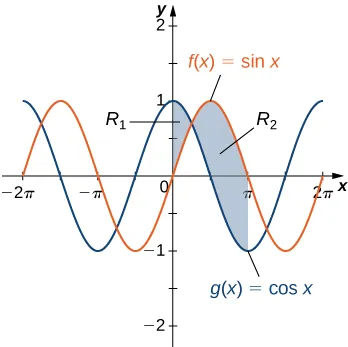
\includegraphics[scale=0.5]{./figures/51be43c1-417e-4df2-a3d0-7d6ec562ccb2.png}
        \end{center}
    \end{minipage}
    \begin{minipage}{0.47\textwidth}
        By theorem 2, we can find the area $A$, in the region $R$ with the following integral:
        \begin{align*}
            &\int_{a}^{b}\ \abs{f(x)-g(x)}\ dx \\
            &=\int_{0}^{\pi}\ \abs{\sin{x}-\cos{x}}\ dx \\
        .\end{align*}
        First, we need to find where the sign of the expression changes:
        \begin{align*}
            &=\sin{x} - \cos{x} = 0 \\
            &=\frac{\sin{x}}{\cos{x}} = \frac{\cos{x}}{\cos{x}} \\
            &=\tan{x} = 1 \\
            &x = \tan^{-1}{1},\ \quad \bigg(-\frac{\pi}{2},\frac{\pi}{2}\bigg) \\
            &x= \frac{\pi}{4}
        .\end{align*}
    \end{minipage}
    \pagebreak \bigbreak \noindent 
    \begin{minipage}{0.47\textwidth}
        Thus:
           \begin{equation}
            \sin{x} - \cos{x}=
                \begin{cases}
                     \sin{x}-\cos{x}& \text{if } x \geq \frac{\pi}{4} \\
                     -(\sin{x}-\cos{x})& \text{if } x < \frac{\pi}{4} 
                \end{cases}
            \end{equation}
    \end{minipage}
    \begin{minipage}[t]{0.47\textwidth}
        So our integral is now:
        \begin{align*}
            &\int_{0}^{\frac{\pi}{4}}\ -(\sin{x}-\cos{x}) dx + \int_{\frac{\pi}{4}}^{\pi}\ \sin{x}-\cos{x}\ dx \\
            &=\int_{0}^{\frac{\pi}{4}}\ \cos{x}-\sin{x}\ dx + \int_{\frac{\pi}{4}}^{\pi}\ \sin{x}-\cos{x}\ dx \\
            &Where:\ I_{1} = \int_{0}^{\frac{\pi}{4}}\ \cos{x}-\sin{x}\ dx \\
            &I_{2} = \int_{\frac{\pi}{4}}^{\pi}\ \sin{x}-\cos{x}\ dx \\
            &A = I_{1} + I_{2}
        .\end{align*}
    \end{minipage}
    \bigbreak \noindent 
    \begin{minipage}[t]{0.47\textwidth}
        Computing both integrals we get:
    \end{minipage}
    \begin{minipage}[t]{0.47\textwidth}
    
    \begin{align*}
        &I_{1} = \int_{0}^{\frac{\pi}{4}}\ \cos{x}-\sin{x}\ dx \\
        &=\sin{x} + \cos{x}\bigg]^{0}_{\frac{\pi}{4}} \\
        &= \bigg(\sin{\bigg(\frac{\pi}{4}\bigg)+\cos{\bigg(\frac{\pi}{4}\bigg)}}\bigg) - \bigg(\sin{(0)+\cos{0}}\bigg)\\
        &= \sqrt{2} - 1
    .\end{align*}
    \begin{align*}
        &=I_{2} = \int_{\frac{\pi}{4}}^{\pi}\ \sin{x}-\cos{x}\ dx \\
        &= -\cos{x}-\sin{x}\bigg]^{\frac{\pi}{4}}_{\pi} \\
        &= - \bigg[\cos{x}+\sin{x}\bigg]^{\pi}_{\frac{\pi}{4}} \\
        &= - \bigg[\bigg(\cos{\pi}+\sin{\pi}\bigg) - \bigg(\cos{\bigg(\frac{\pi}{4}\bigg)+\sin{\bigg(\frac{\pi}{4}\bigg)}}\bigg)\bigg] \\
        &= - \bigg[-1 - \sqrt{2}\bigg] \\
        &= 1 + \sqrt{2}
    .\end{align*}
    \end{minipage}
    \bigbreak \noindent 
    \begin{minipage}[t]{0.47\textwidth}
        Thus:
    \end{minipage}
    \begin{minipage}[t]{0.22\textwidth}
        \begin{align*}
        &A = I_{1} + I_{2} \\
        &= \sqrt{2} - 1 + 1 + \sqrt{2} \\
        & = 2\sqrt{2}\ \ \ Units^{2}
    .\end{align*}
    \end{minipage}

    \pagebreak 
    \phantomsection
    \addcontentsline{toc}{subsection}{Finding the Area of a Complex Region}
    \subsection*{Finding the Area of a Complex Region}
    \bigbreak \noindent 
    \begin{definition}
    \textbf{a "complex region" between curves usually refers to an area that is not easily described by a single, continuous function over the interval of interest.} 
    \end{definition}
    \bigbreak \noindent 
    Consider the following example:
    \bigbreak \noindent 
    \begin{eg}
        If \( R \) is the region between the graphs of the functions \( f(x) = x^{2} \) and \( g(x) = 2-x \) over the interval \([0, 2]\), find the area of region \( R \).
    \end{eg}
    \bigbreak \noindent 
    \begin{minipage}{0.47\textwidth}
        \bigbreak \noindent 
        \textit{Figure 2.7}
        \begin{center}
            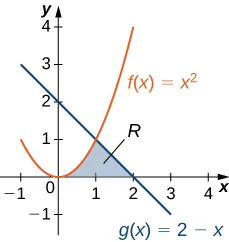
\includegraphics[scale=0.7]{ ./figures/graph4.png }
        \end{center}
    \end{minipage}
    \begin{minipage}{0.47\textwidth}
        As with Example 2.3, we need to divide the interval into two pieces. The graphs of the functions intersect at \( x=1 \) (set \( f(x)=g(x) \) and solve for \( x \)), so we evaluate two separate integrals: one over the interval \([0,1]\) and one over the interval \([1,2]\).
        \bigbreak \noindent 
        Over the interval \([0,1]\), the region is bounded above by \( f(x)=x^2 \) and below by the x-axis, so we have
        \[
        A_1 = \int_{0}^{1} x^2 \, dx = \left. \frac{x^3}{3} \right|_{0}^{1} = \frac{1}{3}.
        \]

        Over the interval \([1,2]\), the region is bounded above by \( g(x)=2-x \) and below by the x-axis, so we have
        \[
        A_2 = \int_{2}^{1} (2-x) \, dx = \left[ 2x - \frac{x^2}{2} \right]_{2}^{1} = \frac{1}{2}.
        \]

        Adding these areas together, we obtain
        \[
        A = A_1 + A_2 = \frac{1}{3} + \frac{1}{2} = \frac{5}{6}.
        \]
        The area of the region is \( \frac{5}{6} \) \text{units}^2.
    \end{minipage}

    \pagebreak
    \phantomsection
    \addcontentsline{toc}{subsection}{Regions Defined with Respect to y}
    \subsection*{Regions Defined with Respect to y}
    \bigbreak \noindent 
    In Example 3, we had to evaluate two separate integrals to calculate the area of the region. However, there is another approach that requires only one integral. What if we treat the curves as functions of \( y \), instead of as functions of \( x \)?
    \bigbreak \noindent 
    Review Figure 2.7. Note that the left graph, shown in red, is represented by the function \( y = f(x) = x^2 \).
    We could just as easily solve this for \( x \) and represent the curve by the function \( x = v(y) = \sqrt{y} \).
    \bigbreak \noindent 
    \nt{(Note that \( x = -\sqrt{y} \) is also a valid representation of the function \( y = f(x) = x^2 \) as a function of \( y \). However, based on the graph, it is clear we are interested in the positive square root.)}
    \bigbreak \noindent 
    Similarly, the right graph is represented by the function \( y = g(x) = 2 - x \), but could just as easily be represented by the function \( x = u(y) = 2 - y \).
    \bigbreak \noindent 
    When the graphs are represented as functions of $y$, we see the region is bounded on the left by the graph of one function and on the right by the graph of the other function. Therefore, if we integrate with respect to $y$, we need to evaluate one integral only. Let’s develop a formula for this type of integration.
    \bigbreak \noindent \bigbreak \noindent  
    \begin{minipage}{0.47\textwidth}
        \begin{center}
            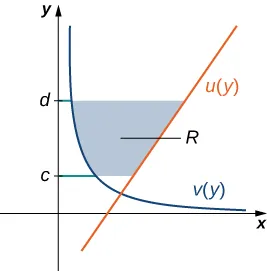
\includegraphics[scale=0.6]{./figures/graph5.png}
        \end{center}
    \end{minipage}
    \begin{minipage}{0.47\textwidth}
        Let \( u(y) \) and \( v(y) \) be continuous functions over an interval \([c, d]\) such that \( u(y) \geq v(y) \) for all \( y \in [c, d] \). We want to find the area between the graphs of the functions, as shown in the following figure.
    \end{minipage}
    \bigbreak \noindent 
    \begin{minipage}{0.47\textwidth}
        \bigbreak \noindent 
        \textit{Figure 2.9}
        \begin{center}
            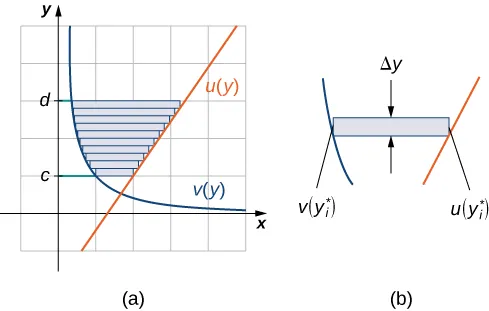
\includegraphics[scale=.45]{./figures/graph6.png }
        \end{center} 
    \end{minipage}
    \begin{minipage}{0.47\textwidth}
        This time, we are going to partition the interval on the \( y \)-axis and use horizontal rectangles to approximate the area between the functions. So, for \( i = 0, 1, 2, \ldots, n \), let \( Q = \{ y_i \} \) be a regular partition of \([c, d]\). Then, for \( i = 1, 2, \ldots, n \), choose a point \( y^*_i \in [y_{i-1}, y_i] \), then over each interval \([y_{i-1}, y_i]\) construct a rectangle that extends horizontally from \( v(y^*_i) \) to \( u(y^*_i) \).
    %\caption{}
    %\label{fig:}
    \end{minipage}
    \bigbreak \noindent 
    \nt{Figure 2.9(a) shows the rectangles when \( y^*_i \) is selected to be the lower endpoint of the interval and \( n = 10 \).
        Figure 2.9(b) shows a representative rectangle in detail.
}
    \pagebreak \bigbreak \noindent 
    The height of each individual rectangle is \( \Delta y \) and the width of each rectangle is \( u(y^*_i) - v(y^*_i) \). Therefore, the area between the curves is approximately
    \[
    A \approx \sum_{i=1}^{n} [u(y^*_i) - v(y^*_i)] \Delta y
    \]
    This is a Riemann sum, so we take the limit as \( n \to \infty \), obtaining
    \[
    A = \lim_{{n \to \infty}} \sum_{i=1}^{n} [u(y^*_i) - v(y^*_i)] \Delta y = \int_{c}^{d} [u(y) - v(y)] \, dy
    \]
    These findings are summarized in the following theorem.
    \bigbreak \noindent 
    \begin{thrm}[Area between two curves, integrating on the y-axis]
       Let \( u(y) \) and \( v(y) \) be continuous functions such that \( u(y) \geq v(y) \) for all \( y \in [c, d] \). Let \( R \) denote the region bounded on the right by the graph of \( u(y) \), on the left by the graph of \( v(y) \), and above and below by the lines \( y = d \) and \( y = c \), respectively. Then, the area of \( R \) is given by
        \[
        A = \int_{c}^{d} [u(y) - v(y)] \, dy
        \] 
    \end{thrm}

    \pagebreak 
    \phantomsection
    \addcontentsline{toc}{section}{2.2 Determining Volumes by Slicing}
    \section*{2.2 Determining Volumes by Slicing}
    \bigbreak \noindent 
    \phantomsection
    \addcontentsline{toc}{subsection}{Volume and the Slicing Method}
    \subsection*{Volume and the Slicing Method}
    \bigbreak \noindent 
    Just as area is the numerical measure of a two-dimensional region, volume is the numerical measure of a three-dimensional solid. Most of us have computed volumes of solids by using basic geometric formulas. The volume of a rectangular solid, for example, can be computed by multiplying length, width, and height: \( V = l \times w \times h \).
    \bigbreak \noindent 
    The formulas for the volume of a sphere \(\left( V = \frac{4}{3} \pi r^3 \right)\),
    a cone \(\left( V = \frac{1}{3} \pi r^2 h \right)\),
    and a pyramid \(\left( V = \frac{1}{3} A h \right)\)
    have also been introduced. Although some of these formulas were derived using geometry alone, all these formulas can be obtained by using integration.
    \bigbreak \noindent 
    We can also calculate the volume of a cylinder. Although most of us think of a cylinder as having a circular base, such as a soup can or a metal rod, in mathematics the word cylinder has a more general meaning. To discuss cylinders in this more general context, we first need to define some vocabulary.
    \bigbreak \noindent 
    \begin{definition}
        We define the \textbf{cross-section} of a solid to be the intersection of a plane with the solid. A \textbf{cylinder} is defined as any solid that can be generated by translating a plane region along a line perpendicular to the region, called the \textbf{axis} of the cylinder. Thus, all cross-sections perpendicular to the axis of a cylinder are identical. 
        \bigbreak \noindent 
        In the case of a right circular cylinder (soup can), this becomes \( V = \pi r^2 h \).
    \end{definition}
    \bigbreak \noindent 
    The solid shown in Figure 2.11 is an example of a cylinder with a noncircular base. To calculate the volume of a cylinder, then, we simply multiply the area of the cross-section by the height of the cylinder: \( V = A \cdot h \).
    \bigbreak \noindent 
    \textit{Figure 2.11}
    \begin{center}
        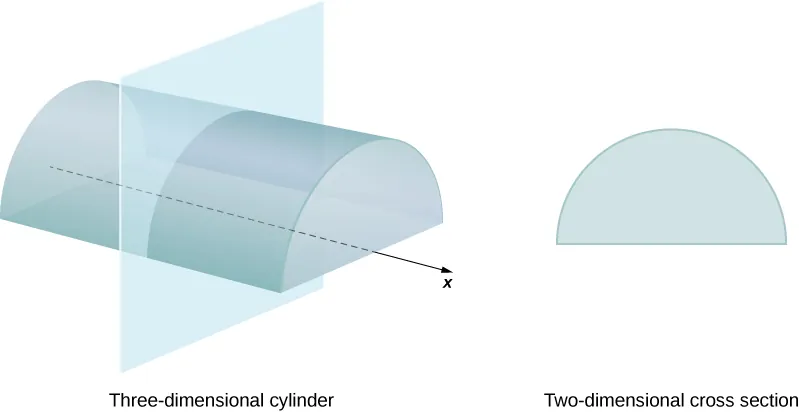
\includegraphics[scale=.6]{./figures/graph8.png}
    \end{center}

    \pagebreak \bigbreak \noindent 
    If a solid does not have a constant cross-section (and it is not one of the other basic solids), we may not have a formula for its volume. In this case, we can use a definite integral to calculate the volume of the solid. We do this by slicing the solid into pieces, estimating the volume of each slice, and then adding those estimated volumes together. The slices should all be parallel to one another, and when we put all the slices together, we should get the whole solid. Consider, for example, the solid S shown in Figure 2.12, extending along the x-axis.
    \bigbreak \noindent 
    \textit{\textbf{Figure 2.12} A solid with a varying cross-section.}
    \bigbreak \noindent 
    \begin{center}
        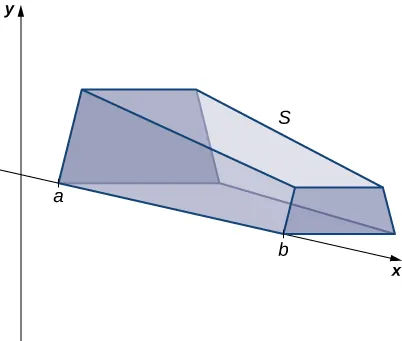
\includegraphics[scale=0.6]{./figures/graph9.png}
    \end{center}
    \bigbreak \noindent 
    We want to divide \( S \) into slices perpendicular to the \( x \)-axis. As we see later in the chapter, there may be times when we want to slice the solid in some other direction---say, with slices perpendicular to the \( y \)-axis. The decision of which way to slice the solid is very important. If we make the wrong choice, the computations can get quite messy. Later in the chapter, we examine some of these situations in detail and look at how to decide which way to slice the solid. For the purposes of this section, however, we use slices perpendicular to the \( x \)-axis.
    \bigbreak \noindent 
    Because the cross-sectional area is not constant, we let \( A(x) \) represent the area of the cross-section at point \( x \). Now let \( P = \{ x_0, x_1, \ldots, x_n \} \) be a regular partition of \([a, b]\), and for \( i = 1, 2, \ldots, n \), let \( S_i \) represent the slice of \( S \) stretching from \( x_{i-1} \) to \( x_i \). The following figure shows the sliced solid with \( n = 3 \).
    \bigbreak \noindent 
    \begin{center}
        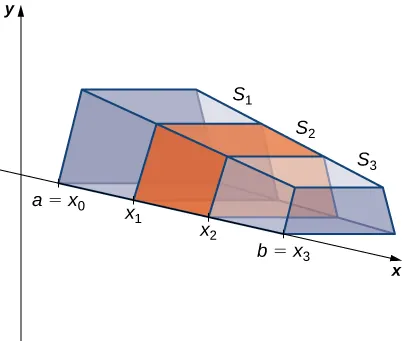
\includegraphics[scale=0.6]{./figures/graph10.png}
    \end{center}
    \pagebreak \bigbreak \noindent 
    Finally, for \( i = 1, 2, \ldots, n \),
    let \( x^*_i \) be an arbitrary point in \([x_{i-1}, x_i]\).
    Then the volume of slice \( S_i \)
    can be estimated by \( V(S_i) \approx A(x^*_i) \Delta x \).
    Adding these approximations together, we see the volume of the entire solid \( S \)
    can be approximated by
    \begin{align*}
        V(s) = \summation{n}{i=1}\ A(x_{i}^{*})\ \Delta x 
    .\end{align*}
    \bigbreak \noindent 
    By now, we can recognize this as a Riemann sum, and our next step is to take the limit as  $n \rightarrow \infty$. Thus, we have:
    \begin{align*}
        V(s) = \summation{n}{i=1}\ A(x_{i}^{*})\ \Delta x  = \int_{a}^{b}\ A(x)\ dx
    .\end{align*}
    \bigbreak \noindent 
    Thus, we can summarize our findings as:
    \begin{thrm}[Slicing Method]
        \begin{align*}
            V(s) = \summation{n}{i=1}\ A(x_{i}^{*})\ \Delta x  = \int_{a}^{b}\ A(x)\ dx
        .\end{align*}
    \end{thrm}
    
    \bigbreak \noindent 
    \begin{definition}
        The technique we have just described is called the \textbf{slicing method}. To apply it, we use the following strategy.
        \begin{enumerate}
            \item Examine the solid and determine the shape of a cross-section of the solid. It is often helpful to draw a picture if one is not provided.
            \item Determine a formula for the area of the cross-section.
            \item Integrate the area formula over the appropriate interval to get the volume.
        \end{enumerate}
    \end{definition}
    \bigbreak \noindent 
    \nt{For now, we assume the slices are perpendicular to the  x-axis. Therefore, the area formula is in terms of x and the limits of integration lie on the  x-axis. However, the problem-solving strategy shown here is valid regardless of how we choose to slice the solid.}

    \pagebreak \bigbreak \noindent 

    \begin{eg}[Deriving the Formula for the Volume of a Pyramid]
        We know from geometry that the formula for the volume of a pyramid is  $V = \frac{1}{3}Ah$ 
        If the pyramid has a square base, this becomes  $V=\frac{1}{3}a^{2}h $ where $a$ 
        denotes the length of one side of the base. We are going to use the slicing method to derive this formula.
    \end{eg}
    \bigbreak \noindent 
    \textbf{Solution:}
    \bigbreak \noindent 
    We want to apply the slicing method to a pyramid with a square base. To set up the integral, consider the pyramid shown in Figure 2.14, oriented along the  x-axis.
    \bigbreak \noindent 
    \textit{\textbf{Figure 2.14:} A pyramid with a square base is oriented along the x-axis. (b) A two-dimensional view of the pyramid is seen from the side.}
    \begin{center}
        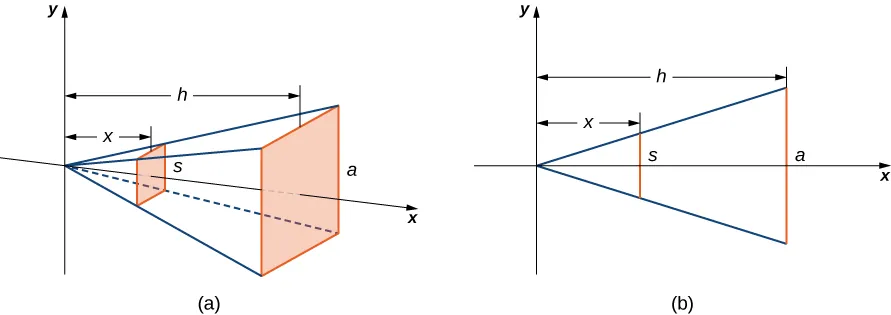
\includegraphics[scale=0.5]{./figures/graph11.png}
    \end{center}
    \bigbreak \noindent 
    We first want to determine the shape of a cross-section of the pyramid. We know the base is a square, so the cross-sections are squares as well (step 1). Now we want to determine a formula for the area of one of these cross-sectional squares. Looking at Figure 2.14(b), and using a proportion, since these are similar triangles, we have
    \begin{align*}
        \frac{s}{a} = \frac{x}{h} \quad s = \frac{ax}{h}
    .\end{align*}
    \bigbreak \noindent 
    Therefore, the area of one of the cross-sectional squares is
    \begin{align*}
        A(x) = s^{2} = \bigg(\frac{ax}{h}\bigg)^{2} \quad \text{(Step 2.)}
    .\end{align*}
    \bigbreak \noindent 
    Then we find the volume of the pyramid by integrating from  0 to $h$ (step  3):
    \begin{align*}
        &V = \int_{0}^{h}\ A(x)\ dx \\
        &=\int_{0}^{h}\ \bigg(\frac{ax}{h}\bigg)^{2}\ dx \\
        &=\int_{0}^{h}\ \frac{a^{2}x^{2}}{h^{2}}\ dx\\
        &=\frac{a^{2}}{h^{2}}\int_{0}^{h}\ x^{2}\ dx \\
        &=\bigg[\frac{a^{2}}{h^{2}}\bigg(\frac{1}{3}x^{3}\bigg)\bigg]^{0}_{h} \\
        &=\frac{1}{3}a^{2}h
    .\end{align*}
    \bigbreak \noindent 
    This is the formula we were looking for.
    \pagebreak \bigbreak \noindent 
    \begin{eg}
        Use the slicing method to derive the formula for the volume of a cone ($V = \frac{1}{3}\pi r^{2}h$)
    \end{eg}
    \bigbreak \noindent 
    Let's begin by construing a diagram:
    \bigbreak \noindent 
    \begin{minipage}[]{0.47\textwidth}
        \incfig{conefig}
    \end{minipage}
    \begin{minipage}[]{0.47\textwidth}
    Now our goal is find a function $A(x)$, which represents the area of the cross section (in this case, a circle), as our cross section gets smaller and smaller.
    Then, like we did with the square pyramid, we can use the fact that these our similar triangles to find the equation for $r$. Thus:
    \begin{align*}
        &\frac{r}{x} = \frac{R}{h} \\
        &r = \frac{Rx}{h}
    .\end{align*}
    Since we know that the area of a circle is $\pi r^{2}$, we can deduce that our $A(x)$ will be:
    \begin{align*}
        &A(x) = \pi r^{2} \\
        &A(x) = \pi \bigg(\frac{Rx}{h}\bigg)^{2}
    .\end{align*}
    \end{minipage}
    \bigbreak \noindent 
    \bigbreak \noindent 
    Now by the slice method, which states: $V  = \int_{a}^{b}\ A(x)\ dx $, we have:
    \begin{align*}
        &V = \int_{0}^{h}\ \pi \bigg(\frac{Rx}{h}\bigg)^{2}\ dx \\
        &V = \int_{0}^{h}\ \pi \frac{R^{2}x^{2}}{h^{2}}\ dx \\
        &V = \frac{\pi R^{2}}{h^{2}}\int_{0}^{h}\ x^{2}\ dx \\
        &= \frac{\pi R^{2}}{h^{2}}\bigg[\frac{1}{3}x^{3}\bigg]^{0}_{h} \\
        &= \frac{\pi R^{2}}{h^{2}}\bigg(\frac{1}{3}h^{3}\bigg) \\
        &= \frac{1}{3}\pi R^{2}h 
    .\end{align*}

    \pagebreak \bigbreak \noindent 
    \begin{eg}
        Use the slice method to derive the formula for the volume of a sphere ($v=\frac{4}{3}\pi r^{3}$):    
    \end{eg}
    \bigbreak \noindent 
    First, let's draw a diagram.
    \bigbreak \noindent 
    \begin{minipage}[]{0.47\textwidth}
        \incfig{sphere6}
    \end{minipage}
    \begin{minipage}[]{0.47\textwidth}
        We can see that our cross sections are circles, from this observation we can acknowledge the fact that the area of a circle is $\pi r^{2}$, and our goal is to find an equation for the area of the cross section. To do this we must find an equation for the radius of the cross section. If we draw a line connecting the radius of the sphere to the radius of the cross section, we will see that we have a right triangle, thus enabling us to use Pythagoras's theorem to solve for the radius of the cross section
    \end{minipage}
    \bigbreak \noindent 
    \begin{minipage}[]{0.47\textwidth}
        \incfig{sphere}
    \end{minipage}
    \begin{minipage}[]{0.47\textwidth}
        We see that this figure demonstrates this. Therefore:
        \begin{align*}
            &x^{2} + y^{2} = r^{2} \\
            &x^{2} = r^{2} - y^{2} \\
            &x = \sqrt{r^{2}-y^{2}}
        .\end{align*}
        \bigbreak \noindent 
        Which means the area function for the cross section  is:
        \begin{align*}
            &A(x) =\pi \bigg(\sqrt{r^{2}-y^{2}}\bigg)^{2} \\
            &= \pi \bigg(r^{2}-y^{2}\bigg)
        .\end{align*}
    \end{minipage}
    \bigbreak \noindent 
    From this, using the slicing method, which states, $V = \int_{a}^{b}\ A(x)\ dx $, we get:
    \begin{align*}
        &V= \int_{a}^{b}\ \pi \bigg(r^{2}-y^{2}\bigg)\ dy \\
        &= \int_{-r}^{r}\ \pi \bigg(r^{2}-y^{2}\bigg)\ dy \\
        &= \int_{-r}^{r}\ \pi r^{2} - \pi y^{2}\ dy \\
        &= \pi r^{2}y - \frac{1}{3}\pi y^{3}\bigg]^{r}_{-r} \\
        &= \bigg(\pi r^{2}(r)-\frac{1}{3}\pi(r)^{3}\bigg) - \bigg(\pi r^{2}(-r)-\frac{1}{3}\pi(-r)^{3}\bigg) \\
        &= \bigg(\frac{2\pi r^{3}}{3}\bigg) - \bigg(- \frac{2\pi r^{3}}{3}\bigg) \\
        &= \frac{4}{3}\pi r^{3}
    .\end{align*}
    

    \pagebreak 
    \phantomsection
    \addcontentsline{toc}{subsection}{Solids of Revolution}
    \subsection*{Solids of Revolution}
    \bigbreak \noindent 
    \smallbreak \noindent
    \begin{definition}
        If a region in a plane is revolved around a line in that plane, the resulting solid is called a \textbf{solid of revolution}, as shown in the following figure.
    \end{definition}
    \bigbreak \noindent 
    \begin{minipage}[]{0.47\textwidth}
        \textit{Figure:}
        \bigbreak \noindent 
        \begin{center}
            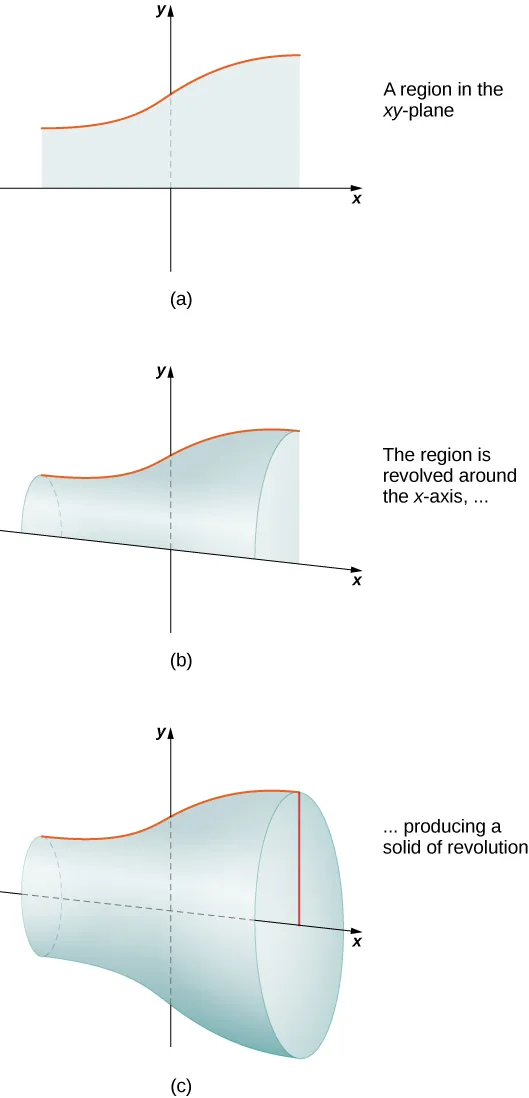
\includegraphics[scale=.4]{./figures/graph20.png}
        \end{center}
        \bigbreak \noindent 
        \nt{Solids of revolution are common in mechanical applications, such as machine parts produced by a lathe. We spend the rest of this section looking at solids of this type. The next example uses the slicing method to calculate the volume of a solid of revolution.}
    \end{minipage}
    \begin{minipage}[]{0.47\textwidth}
        \begin{eg}
            Use the slicing method to find the volume of the solid of revolution bounded by the graphs of  $f(x)=x^{2}-4x+5$, $x=1$, and $x=4$, and rotated about the  x-axis.
            Using the Slicing Method to find the Volume of a Solid of Revolution
        \end{eg}
        \bigbreak \noindent 
        \textbf{Solution:}
        Using the problem-solving strategy, we first sketch the graph of the quadratic function over the interval  [1,4]. We then revolve it around the $x$-axis
        \bigbreak \noindent 
        \begin{center}
            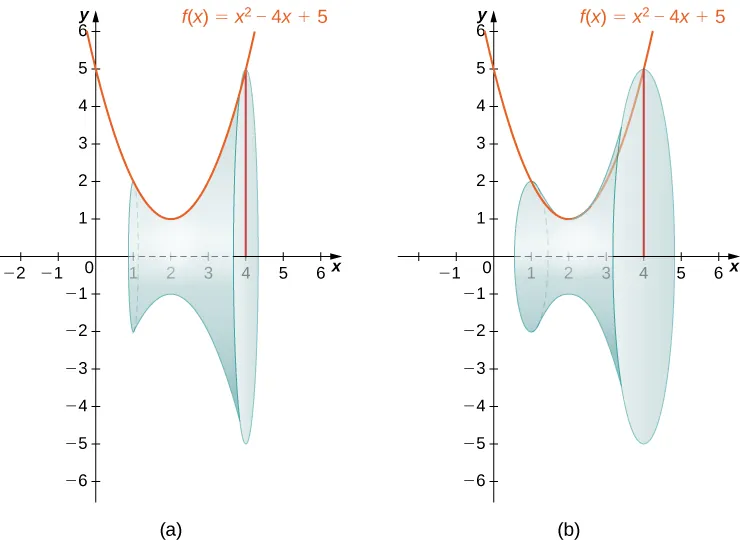
\includegraphics[scale=0.2]{./figures/graph21.png}
        \end{center}
        \bigbreak \noindent 
        Since the solid was formed by revolving the region around the  x-axis,
  the cross-sections are circles (step 1). The area of the cross-section, then, is the area of a circle, and the radius of the circle is given by  f(x).
  Use the formula for the area of the circle:
  \begin{align*}
      A(x) = \pi r^{2} = \pi\big[f(x)\big]^{2} = \pi(x^{2}-4x+5)^{2}
  .\end{align*}
  The volume is then:
  \begin{align*}
      &V = \int_{a}^{b} A(x)\ dx  \\
      &= \int_{4}^{1} \pi (x^2 - 4x + 5)^2\ dx  \\
      &= \pi \int_{4}^{1} (x^4 - 8x^3 + 26x^2 - 40x + 25)\ dx  \\
      &= \pi \left[ \frac{x^5}{5} - 2x^4 + \frac{26x^3}{3} - 20x^2 + 25x \right]_{1}^{4} = \frac{78}{5}\pi.
  .\end{align*}
    \end{minipage}

    \pagebreak 
    \phantomsection
    \addcontentsline{toc}{subsection}{The Disk Method}
    \subsection*{The Disk Method}
    \bigbreak \noindent 
    \smallbreak \noindent
    \begin{definition}
            When we use the slicing method with solids of revolution, it is often called the \textit{disk method} because, for solids of revolution, the slices used to over approximate the volume of the solid are disks. To see this, consider the solid of revolution generated by revolving the region between the graph of the function \( f(x) = (x - 1)^{2} + 1 \) and the \( x \)-axis over the interval \([ -1, 3 ]\) around the \( x \)-axis. The graph of the function and a representative disk are shown in Figure 2.18(a) and (b). The region of revolution and the resulting solid are shown in Figure 2.18(c) and (d).
    \end{definition}
    \bigbreak \noindent 
    \begin{center}
        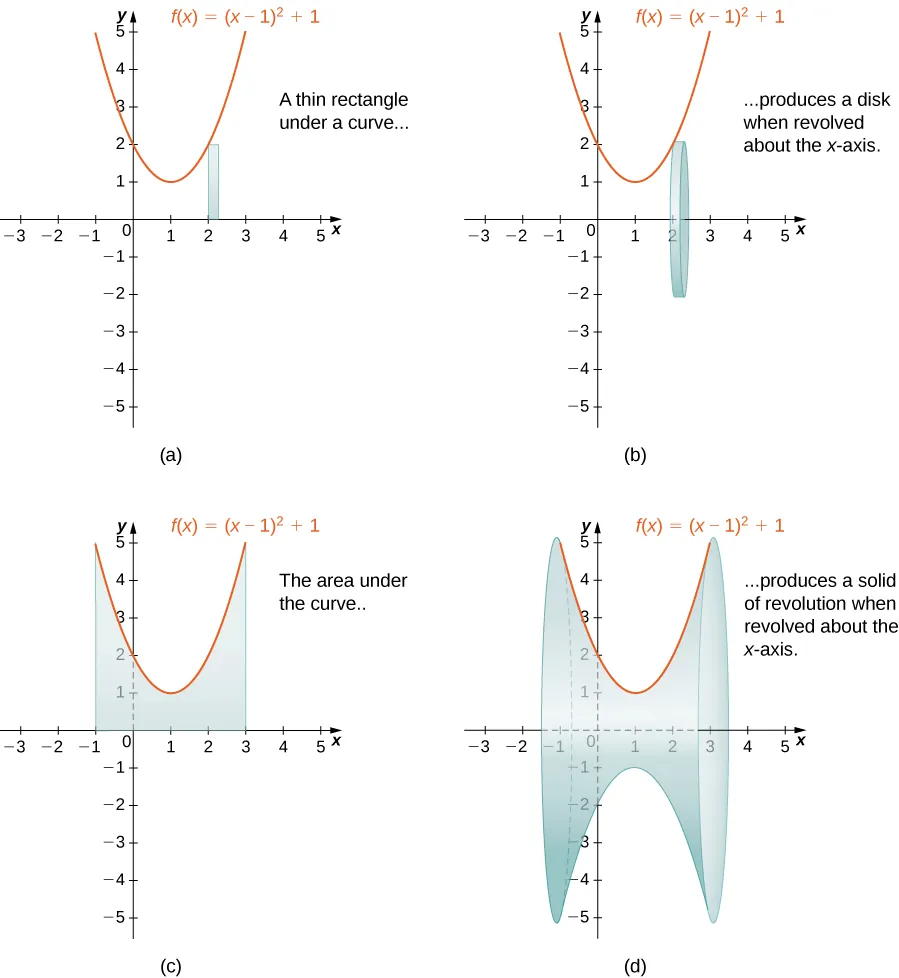
\includegraphics[scale=0.5]{./figures/graph22.png}
    \end{center}

    \pagebreak \bigbreak \noindent 
    We already used the formal Riemann sum development of the volume formula when we developed the slicing method. We know that
    \[
    V = \int_{a}^{b} A(x) \, dx.
    \]
    The only difference with the \textit{disk method} is that we know the formula for the cross-sectional area ahead of time; it is the area of a circle. This gives the following rule.
    \bigbreak \noindent 
    \begin{thrm}[Disk Method Along the x-axis]
       Let \( f(x) \) be continuous and nonnegative. Define \( R \) as the region bounded above by the graph of \( f(x) \), below by the \( x \)-axis, on the left by the line \( x = a \), and on the right by the line \( x = b \). Then, the volume of the solid of revolution formed by revolving \( R \) around the \( x \)-axis is given by
        \[
        V = \int_{a}^{b} \pi [f(x)]^2 \, dx.
        \] 
    \end{thrm}
    \bigbreak \noindent 
    we can generate a solid of revolution by revolving a plane region around any horizontal or vertical line. In the next example, we look at a solid of revolution that has been generated by revolving a region around the  $y$-axis.
  The mechanics of the disk method are nearly the same as when the  $x$-axis
  is the axis of revolution, but we express the function in terms of  $y$
  and we integrate with respect to $y$ as well. This is summarized in the following rule.
  \bigbreak \noindent 
  \begin{thrm}[Disk Method Along The y-axis]
    Let \( g(y) \) be continuous and nonnegative. Define \( Q \) as the region bounded on the right by the graph of \( g(y) \), on the left by the \( y \)-axis, below by the line \( y = c \), and above by the line \( y = d \). Then, the volume of the solid of revolution formed by revolving \( Q \) around the \( y \)-axis is given by
    \[
    V = \int_{c}^{d} \pi [g(y)]^2 \, dy.
    \]    
  \end{thrm}
  \bigbreak \noindent 
  \begin{eg}
      Let \( R \) be the region bounded by the graph of \( g(y) = \sqrt{4 - y} \) and the \( y \)-axis over the \( y \)-axis interval \([0, 4]\). Use the \textit{disk method} to find the volume of the solid of revolution generated by rotating \( R \) around the \( y \)-axis.
  \end{eg}
  \bigbreak \noindent 
  \textbf{Solution:} Figure 2.20 shows the function and a representative disk that can be used to estimate the volume. Notice that since we are revolving the function around the  $y$-axis, the disks are horizontal, rather than vertical.
  \bigbreak \noindent 
  \textit{Figure 2.20}
  \begin{center}
      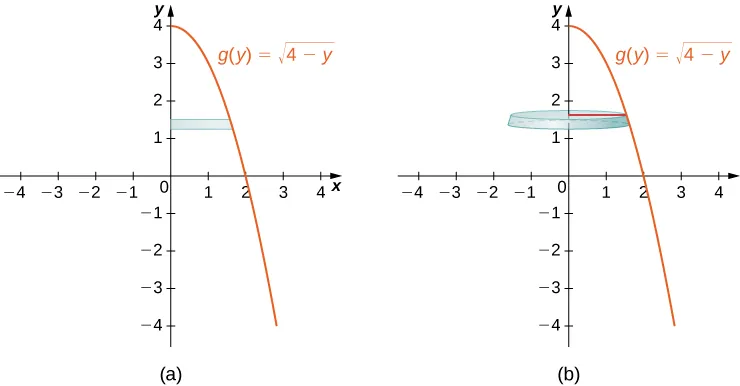
\includegraphics[scale=0.5]{./figures/graph23.png}
  \end{center}
  
    \pagebreak \bigbreak \noindent 
    To find the volume, we integrate with respect to \( y \). We obtain
    \begin{align*}
    &V = \int_{c}^{d} \pi [g(y)]^2\ dy \\
    &= \int_{0}^{4} \pi \left( \sqrt{4 - y} \right)^2\ dy \\
    &= \pi \int_{0}^{4} (4 - y)\ dy \\
    &= \pi \left[ 4y - \frac{y^2}{2} \right]_{0}^{4} \\
    &= 8\pi
    .\end{align*}
    Thus, the volume is \( 8\pi \) units\(^3\).

    \bigbreak \noindent 
    \phantomsection
    \addcontentsline{toc}{subsection}{The Washer Method}
    \subsection*{The Washer Method}
    \bigbreak \noindent 
    Some solids of revolution have cavities in the middle; they are not solid all the way to the axis of revolution. Sometimes, this is just a result of the way the region of revolution is shaped with respect to the axis of revolution. In other cases, cavities arise when the region of revolution is defined as the region between the graphs of two functions. A third way this can happen is when an axis of revolution other than the  $x$-axis or  $y$-axis is selected.
    \bigbreak \noindent 
    When the solid of revolution has a cavity in the middle, the slices used to approximate the volume are not disks, but washers (disks with holes in the center).
    \bigbreak \noindent 
    \begin{minipage}{0.47\textwidth}
        For example, consider the region bounded above by the graph of the function \( f(x) = \sqrt{x} \) and below by the graph of the function \( g(x) = 1 \) over the interval \([1, 4]\). When this region is revolved around the \( x \)-axis, the result is a solid with a cavity in the middle, and the slices are washers. The graph of the function and a representative washer are shown in Figure 2.22(a) and (b). The region of revolution and the resulting solid are shown in Figure 2.22(c) and (d).
        The cross-sectional area, then, is the area of the outer circle less the area of the inner circle. In this case,
        \[
        A(x) = \pi (\sqrt{x})^2 - \pi (1)^2 = \pi (x - 1).
        \]
        Then the volume of the solid is
        \begin{align*}
            &V = \int_{a}^{} A(x)\ dx \\
            &= \int_{1}^{4} \pi (x - 1)\ dx \\
            &= \pi \left[ \frac{x^2}{2} - x \right]_{1}^{4} \\
            &= \frac{9}{2} \pi \text{ units}^3. 
        .\end{align*}
        Generalizing this process gives the \textit{washer method}.
    \end{minipage}
    \begin{minipage}{0.5\textwidth}
        \begin{center}
            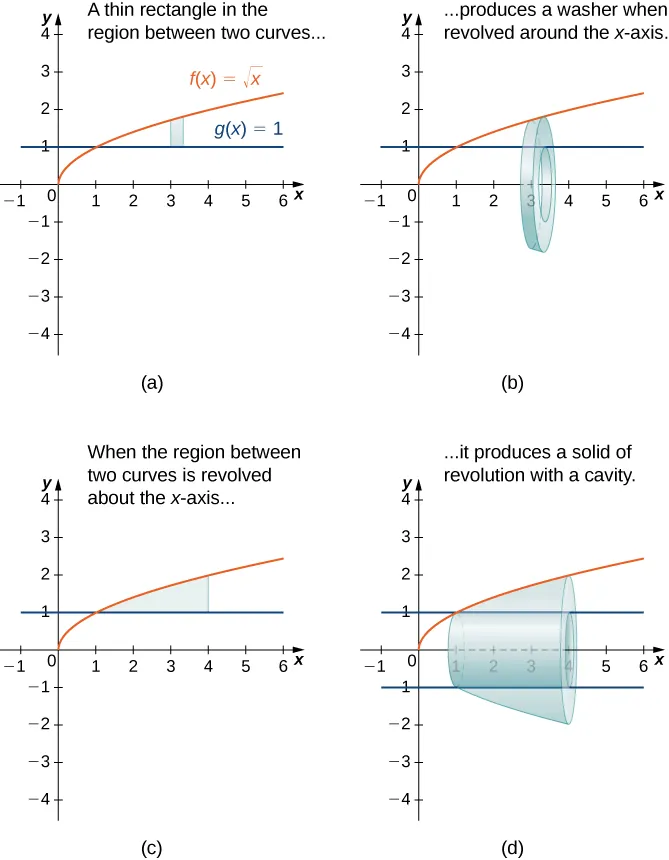
\includegraphics[scale=0.35]{./figures/graph24.png}
        \end{center}
    \end{minipage}

    \pagebreak \bigbreak \noindent 
    \begin{thrm}[The Washer Method]
       Suppose \( f(x) \) and \( g(x) \) are continuous, nonnegative functions such that \( f(x) \geq g(x) \) over \([a, b]\). Let \( R \) denote the region bounded above by the graph of \( f(x) \), below by the graph of \( g(x) \), on the left by the line \( x = a \), and on the right by the line \( x = b \). Then, the volume of the solid of revolution formed by revolving \( R \) around the \( x \)-axis is given by
        \[
        V = \int_{a}^{b} \pi \left[ (f(x))^2 - (g(x))^2 \right] \, dx.
        \] 
    \end{thrm}
    \bigbreak \noindent \bigbreak \noindent 
    As with the disk method, we can also apply the washer method to solids of revolution that result from revolving a region around the y-axis. In this case, the following rule applies.
    \bigbreak \noindent \bigbreak \noindent 
    \begin{thrm}[The washer method, integrating along the y-axis]
        Suppose \( u(y) \) and \( v(y) \) are continuous, nonnegative functions such that \( v(y) \leq u(y) \) for \( y \in [c, d] \). Let \( Q \) denote the region bounded on the right by the graph of \( u(y) \), on the left by the graph of \( v(y) \), below by the line \( y = c \), and above by the line \( y = d \). Then, the volume of the solid of revolution formed by revolving \( Q \) around the \( y \)-axis is given by
        \[
        V = \int_{c}^{d} \pi \left[ (u(y))^2 - (v(y))^2 \right] \, dy.
        \]
    \end{thrm}

    \bigbreak \noindent \bigbreak \noindent 
    \begin{eg}[The Washer Method with a Different Axis of Revolution]
        Find the volume of a solid of revolution formed by revolving the region bounded above by \( f(x) = 4 - x \) and below by the \( x \)-axis over the interval \([0, 4]\) around the line \( y = -2 \).
    \end{eg}
    \bigbreak \noindent 
    \textbf{Solution:} 
    \bigbreak \noindent 
    \begin{minipage}[]{0.47\textwidth}
        \begin{center}
            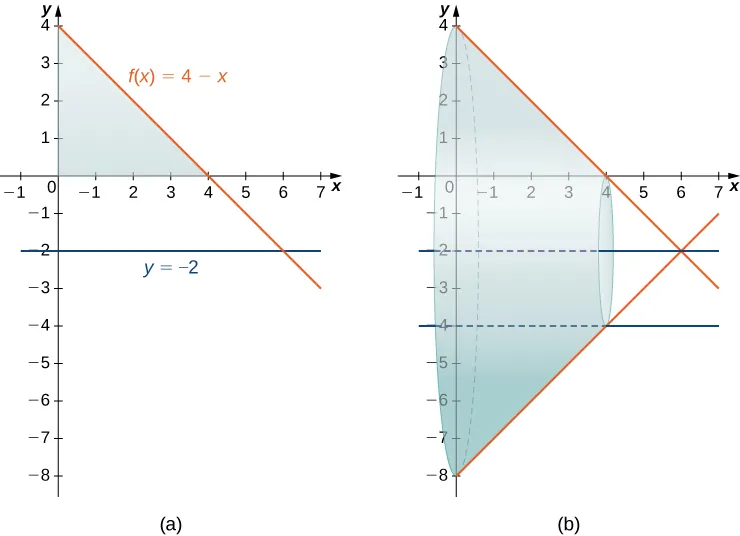
\includegraphics[scale=0.3]{./figures/graph25.png}
        \end{center} 
    \end{minipage}
    \begin{minipage}[]{0.47\textwidth}
        We can’t apply the volume formula to this problem directly because the axis of revolution is not one of the coordinate axes. However, we still know that the area of the cross-section is the area of the outer circle less the area of the inner circle. Looking at the graph of the function, we see the radius of the outer circle is given by  $f(x) +2$,
  which simplifies to:
  \begin{align*}
      &f(x) + 2  \\
      &= (4-x) + 2 \\
      &= 6-x
  .\end{align*}
  The radius of the inner circle is $g(x)=2$, therefore we have:
  \begin{align*}
      &V = \int_{0}^{4}\ \pi \bigg[(6-x)^{2}-(2)^{2}\bigg]\ dx \\
      &=\pi \int_{0}^{4}\ (x^{2}-12x+32)\ dx \\
      &=\pi\bigg[\frac{1}{3}\pi^{3}-6x^{2}+32x\bigg]^{4}_{0} \\
      &=\frac{160\pi}{3}\ \text{ units}^{3}
  .\end{align*}
    \end{minipage}

    \pagebreak 
    \phantomsection
    \addcontentsline{toc}{section}{2.3 Volumes of Revolution: Cylindrical Shells}
    \section*{2.3 Volumes of Revolution: Cylindrical Shells}
    \bigbreak \noindent 
    In this section, we explore the cylindrical shells method for calculating the volume of solids of revolution. Unlike the disk and washer methods, which integrate along the axis parallel to the axis of revolution, this method integrates perpendicularly. This flexibility can simplify calculations for complex functions. The solid's geometry may also make cylindrical shells more advantageous than the washer method. We conclude by summarizing all volume-finding methods and offering guidelines for choosing the appropriate one.
    \smallbreak \noindent
    \phantomsection
    \addcontentsline{toc}{subsection}{The Method of Cylindrical Shells}
    \subsection*{The Method of Cylindrical Shells}
    \bigbreak \noindent 
    \begin{minipage}[]{0.47\textwidth}
           Again, we are working with a solid of revolution. As before, we define a region \( R \),
        bounded above by the graph of a function \( y = f(x) \),
        below by the \( x \)-axis,
        and on the left and right by the lines \( x = a \)
        and \( x = b \),
        respectively, as shown in Figure 2.25(a). We then revolve this region around the \( y \)-axis, as shown in Figure 2.25(b). Note that this is different from what we have done before. Previously, regions defined in terms of functions of \( x \)
        were revolved around the \( x \)-axis
        or a line parallel to it. 
    \end{minipage}
    \begin{minipage}[]{0.47\textwidth}
        \textit{Figure 2.25}
        \begin{center}
            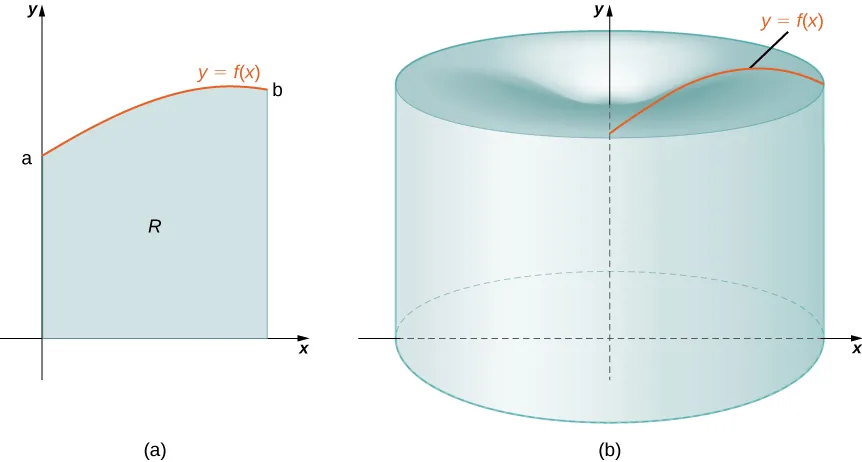
\includegraphics[scale=0.3]{./figures/graph26.png}
        \end{center}
    \end{minipage}
    \bigbreak \noindent 
    \begin{minipage}[]{0.47\textwidth}
        As we have done many times before, partition the interval \([a, b]\)
        using a regular partition, \(P = \{x_0, x_1, \ldots, x_n\}\)
        and, for \(i = 1, 2, \ldots, n\),
        choose a point \(x^*_i \in [x_{i-1}, x_i]\).
        Then, construct a rectangle over the interval \([x_{i-1}, x_i]\)
        of height \(f(x^*_i)\)
        and width \(\Delta x\).
        A representative rectangle is shown in Figure 2.26(a). When that rectangle is revolved around the \(y\)-axis, instead of a disk or a washer, we get a cylindrical shell, as shown in the following figure.
    \end{minipage}
    \begin{minipage}[]{0.47\textwidth}
    \begin{center}
        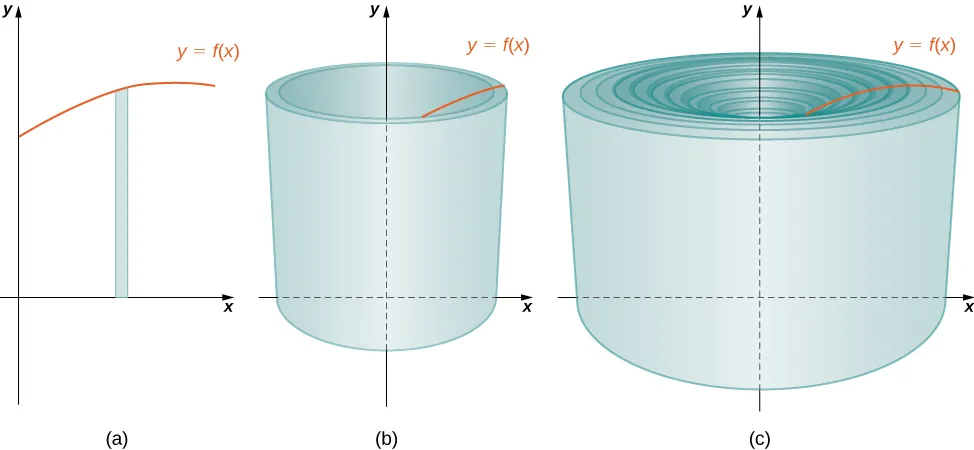
\includegraphics[scale=0.27]{./figures/graph27.png}
    \end{center} 
    \end{minipage}
    \bigbreak \noindent 
    \begin{minipage}[]{0.47\textwidth}
        To calculate the volume of this shell, consider Figure 2.27.
    \end{minipage}
    \begin{minipage}[]{0.47\textwidth}
        \textit{Figure 2.27}
        \begin{center}
            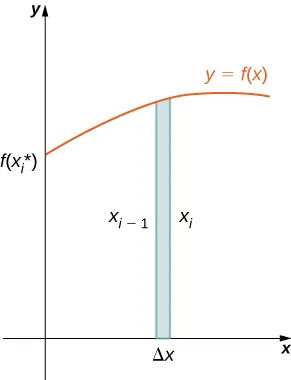
\includegraphics[scale=0.5]{ ./figures/graph28.png }
        \end{center}
    \end{minipage}

    \pagebreak \bigbreak \noindent 
    We know the volume of a cylinder is $\pi r^{2}h $. 
    \bigbreak \noindent 
    The shell is a cylinder, so its volume is the cross-sectional area multiplied by the height of the cylinder. The cross-sections are annuli (ring-shaped regions---essentially, circles with a hole in the center), with outer radius \( x_i \) and inner radius \( x_{i-1} \). Thus, the cross-sectional area is \( \pi x_i^2 - \pi x_{i-1}^2 \). The height of the cylinder is \( f(x^*_i) \). Then the volume of the shell is
    \begin{align*}
    V_{\text{shell}} = f(x^*_i)(\pi x_i^2 - \pi x_{i-1}^2)  \\
    = \pi f(x^*_i)(x_i^2 - x_{i-1}^2)  \\
    = \pi f(x^*_i)(x_i + x_{i-1})(x_i - x_{i-1})  \\
    = 2\pi f(x^*_i)\left(\frac{x_i + x_{i-1}}{2}\right)(x_i - x_{i-1}). \\
    .\end{align*}
    Note that \( x_i - x_{i-1} = \Delta x \), so we have

    \[
    V_{\text{shell}} = 2\pi f(x^*_i)\left(\frac{x_i + x_{i-1}}{2}\right)\Delta x.
    \]
    Furthermore, \( \frac{x_i + x_{i-1}}{2} \) is both the midpoint of the interval \( [x_{i-1}, x_i] \) and the average radius of the shell, and we can approximate this by \( x^*_i \). We then have

    \[
    V_{\text{shell}} \approx 2\pi f(x^*_i) x^*_i \Delta x.
    \]
    \bigbreak \noindent 
    To calculate the volume of the entire solid, we then add the volumes of all the shells and obtain
    \begin{align*}
        V \approx \summation{n}{i=1}\ (2\pi x_{i}^{*}f(x_{i}^{*}))\Delta x\ 
    .\end{align*}
    Here we have another Riemann sum, this time for the function $2\pi xf(x) $ Taking the limit as  $n \rightarrow \infty $ gives us
  \begin{align*}
    V = \lim_{{n \to \infty}} \sum_{{i=1}}^{n} \left( 2\pi x^*_i f(x^*_i) \Delta x \right) = \int_{a}^{b} \left( 2\pi x f(x) \right) dx.
  .\end{align*}
  \bigbreak \noindent 
  This leads to the following rule for the method of cylindrical shells.
  \bigbreak \noindent \bigbreak \noindent 
  \begin{thrm}[The Method of Cylindrical Shells]
      Let \( f(x) \) be continuous and nonnegative. Define \( R \) as the region bounded above by the graph of \( f(x) \), below by the \( x \)-axis, on the left by the line \( x = a \), and on the right by the line \( x = b \). Then the volume of the solid of revolution formed by revolving \( R \) around the \( y \)-axis is given by
      \begin{align*}
          V = \int_{a}^{b}\ (2\pi xf(x))\ dx
      .\end{align*}
  \end{thrm}

  \pagebreak \bigbreak \noindent 
  \begin{eg}
     Define $R$ as the region bounded above by the graph of  $f(x) = \frac{1}{x}$ and below by the  $x$-axis over the interval  $[1,3]$. Find the volume of the solid of revolution formed by revolving  $R$ around the  $y$-axis. 
  \end{eg}
  \bigbreak \noindent 
  \textbf{Solution:} 
  \bigbreak \noindent 
  \begin{minipage}[]{0.47\textwidth}
    First, lets graph the region $R$ and the corresponding solid of revolution: 
    \bigbreak \noindent 
    \begin{center}
        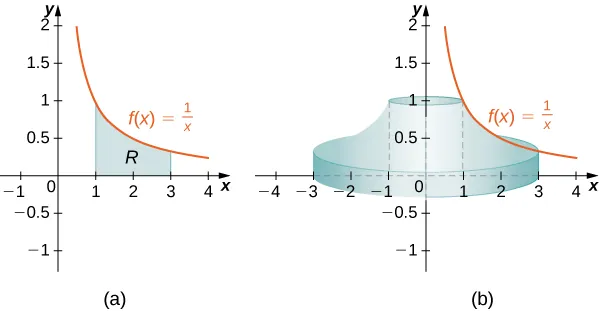
\includegraphics[scale=0.4]{./figures/graph29.png}
    \end{center}
  \end{minipage}
  \begin{minipage}[]{0.47\textwidth}
    Thus, the volume is given by:
    \begin{align*}
        &V = \int_{a}^{b}\ 2\pi xf(x)\ dx \\
        &= \int_{1}^{3}\ 2\pi x\left(\frac{1}{x}\right)\ dx \\
        &= \int_{1}^{3}\ 2\pi \ dx \\ 
        &= 2\pi x\ \bigg|^{3}_1 \\
        &= 2\pi(3) - 2\pi(1) \\
        &= 4\pi\ units^{3}
    .\end{align*}
  \end{minipage}
  \bigbreak \noindent 
  As with the disk method and the washer method, we can use the method of cylindrical shells with solids of revolution, revolved around the  $x$-axis, when we want to integrate with respect to  $y$. The analogous rule for this type of solid is given here.
  \bigbreak \noindent 
  \begin{thrm}[CYLINDRICAL SHELLS FOR S.O.R AROUND THE X-AXIS]
     Let \( g(y) \) be continuous and nonnegative. Define \( Q \) as the region bounded on the right by the graph of \( g(y) \), on the left by the \( y \)-axis, below by the line \( y = c \), and above by the line \( y = d \). Then, the volume of the solid of revolution formed by revolving \( Q \) around the \( x \)-axis is given by
     \begin{align*}
         V = \int_{c}^{d}\ 2\pi y(g(y))\ dy
     .\end{align*}
 
  \end{thrm}

  \pagebreak \bigbreak \noindent 
  \begin{eg}
     Define \( Q \) as the region bounded on the right by the graph of \( g(y) = 2y\sqrt{} \) and on the left by the \( y \)-axis for \( y \in [0, 4] \). Find the volume of the solid of revolution formed by revolving \( Q \) around the \( x \)-axis.
  \end{eg}
  \bigbreak \noindent 
  \textbf{Solution:}
  \bigbreak \noindent 
  \begin{minipage}[]{0.47\textwidth}
      First, we need to graph the region $Q$ and the associated solid of revolution, as shown in the following figure.
      \bigbreak \noindent 
      \begin{center}
          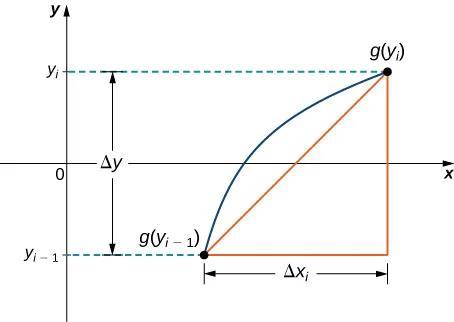
\includegraphics[scale=0.4]{./figures/graph30.png}
      \end{center}
  \end{minipage}
  \begin{minipage}[]{0.47\textwidth}
    Thus, the volume is given by:
    \begin{align*}
        &V = \int_{c}^{d}\ 2\pi yg(y)\ dy \\
        &= \int_{0}^{4}\ 2\pi y \left(2\sqrt{y}\right)\ dy \\
        &= 4\pi \int_{0}^{4}\ y^{\frac{3}{2}}\ dy \\
        &= 4\pi \left[\frac{2}{5}y^{\frac{5}{2}}\right]_0^{4}  \\
        &= 4\pi \left(\frac{2}{5}(4)^{\frac{5}{2}}\right) \\
        &=\frac{256\pi}{5}\ units^{3}
    .\end{align*}
  \end{minipage}
  \bigbreak \noindent 
  For the next example, we look at a solid of revolution for which the graph of a function is revolved around a line other than one of the two coordinate axes. To set this up, we need to revisit the development of the method of cylindrical shells. Recall that we found the volume of one of the shells to be given by
    \[
    V_{\text{shell}} = 2\pi f(x^*_i) \left( \frac{x_i + x_{i-1}}{2} \right) (x_i - x_{i-1}).
    \]
    This was based on a shell with an outer radius of \( x_i \) and an inner radius of \( x_{i-1} \). If, however, we rotate the region around a line other than the \( y \)-axis, we have a different outer and inner radius. Suppose, for example, that we rotate the region around the line \( x = -k \), where \( k \) is some positive constant. Then, the outer radius of the shell is \( x_i + k \) and the inner radius of the shell is \( x_{i-1} + k \). Substituting these terms into the expression for volume, we get
    \begin{align*}
        &V_{\text{shell}} = 2\pi f(x^*_i) \left( \frac{(x_i + k) + (x_{i-1} + k)}{2} \right) ((x_i + k) - (x_{i-1} + k))  \\
        &= 2\pi f(x^*_i) \left( \frac{x_i + x_{i-1}}{2} + k \right) \Delta x.
    .\end{align*}
    As before, we notice that \( \frac{x_i + x_{i-1}}{2} \) is the midpoint of the interval \( [x_{i-1}, x_i] \) and can be approximated by \( x^*_i \). Then, the approximate volume of the shell is
    \[
    V_{\text{shell}} \approx 2\pi (x^*_i + k) f(x^*_i) \Delta x.
    \]
    The remainder of the development proceeds as before, and we see that
    \[
    V = \int_{a}^{b} \left( 2\pi (x + k) f(x) \right) dx.
    \]
    We could also rotate the region around other horizontal or vertical lines, such as a vertical line in the right half plane. In each case, the volume formula must be adjusted accordingly. Specifically, the \( x \)-term in the integral must be replaced with an expression representing the radius of a shell. To see how this works, consider the following example.

    \pagebreak 
    \phantomsection
    \addcontentsline{toc}{subsection}{A Region of Revolution Bounded by the Graphs of Two Functions}
    \subsection*{A Region of Revolution Bounded by the Graphs of Two Functions}
    \bigbreak \noindent 
    \begin{thrm}[A Region of Revolution Bounded by the Graphs of Two Functions]
       \begin{align*}
           V = \int_{a}^{b}\ 2\pi x\left[f(x)-g(x)\right]\ dx
       .\end{align*} 
    \end{thrm}

    \bigbreak \noindent 
    \phantomsection
    \addcontentsline{toc}{subsection}{Which Method Should We Use?}
    \subsection*{Which Method Should We Use?}
    \bigbreak \noindent 
    We have studied several methods for finding the volume of a solid of revolution, but how do we know which method to use? It often comes down to a choice of which integral is easiest to evaluate. Figure 2.34 describes the different approaches for solids of revolution around the  x-axis.
      It’s up to you to develop the analogous table for solids of revolution around the  y-axis.
      \bigbreak \noindent 
      \textit{Figure 2.34:}
      \bigbreak \noindent 
      \begin{center}
          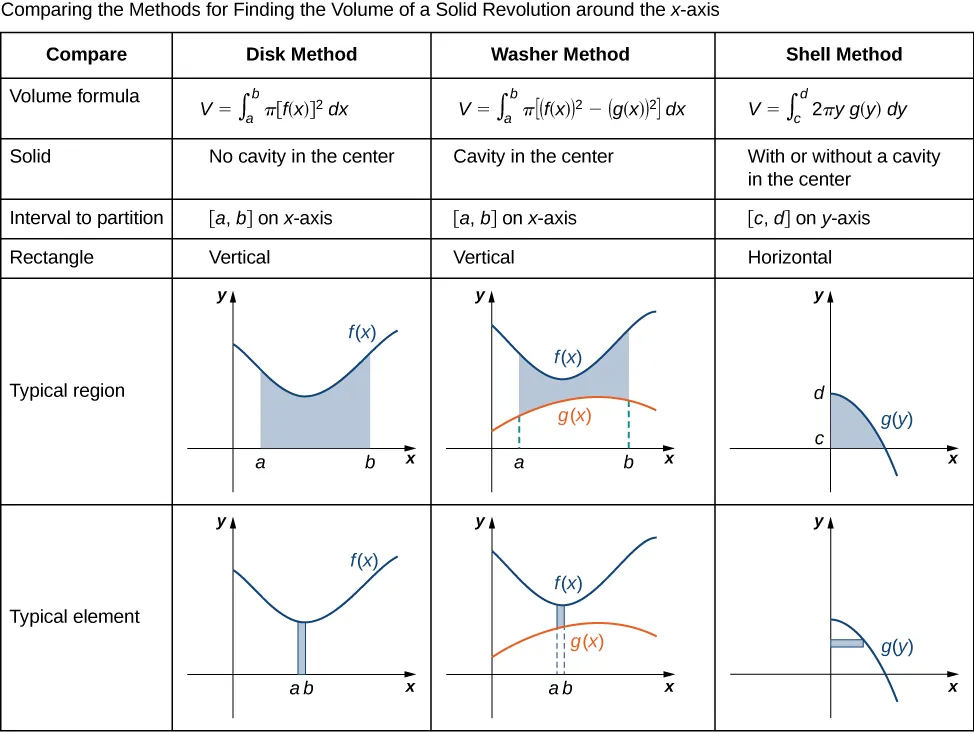
\includegraphics[scale=0.5]{./figures/graph31.png}
      \end{center}

      \pagebreak \bigbreak \noindent 
      \phantomsection
      \addcontentsline{toc}{section}{2.4 Arc Length of a Curve and Surface Area}
      \section*{2.4 Arc Length of a Curve and Surface Area}
      \bigbreak \noindent 
      In this section, we use definite integrals to find the arc length of a curve. We can think of arc length as the distance you would travel if you were walking along the path of the curve. Many real-world applications involve arc length. If a rocket is launched along a parabolic path, we might want to know how far the rocket travels. Or, if a curve on a map represents a road, we might want to know how far we have to drive to reach our destination.
      \bigbreak \noindent 
        We begin by calculating the arc length of curves defined as functions of \(x\), then we examine the same process for curves defined as functions of \(y\). (The process is identical, with the roles of \(x\) and \(y\) reversed.) The techniques we use to find arc length can be extended to find the surface area of a surface of revolution, and we close the section with an examination of this concept.

    \bigbreak \noindent 
    \phantomsection
    \addcontentsline{toc}{subsection}{Arc Length of the Curve y = f(x)}
    \subsection*{Arc Length of the Curve y = f(x)}
    \bigbreak \noindent 
    In previous applications of integration, we required the function \(f(x)\) to be integrable, or at most continuous. However, for calculating arc length, we have a more stringent requirement for \(f(x)\). Here, we require \(f(x)\) to be differentiable, and furthermore, we require its derivative, \(f'(x)\), to be continuous. Functions like this, which have continuous derivatives, are called smooth. (This property comes up again in later chapters.)
    \bigbreak \noindent 
    \begin{minipage}[]{0.47\textwidth}
        Let \(f(x)\) be a smooth function defined over \([a,b]\). We want to calculate the length of the curve from the point \((a,f(a))\) to the point \((b,f(b))\). We start by using line segments to approximate the length of the curve. For \(i=0,1,2,\ldots,n\), let \(P=\{x_i\}\) be a regular partition of \([a,b]\). Then, for \(i=1,2,\ldots,n\), construct a line segment from the point \((x_{i-1},f(x_{i-1}))\) to the point \((x_i,f(x_i))\). Although it might seem logical to use either horizontal or vertical line segments, we want our line segments to approximate the curve as closely as possible. Figure 2.37 depicts this construct for \(n=5\).
    \end{minipage}
    \begin{minipage}[]{0.47\textwidth}
        \begin{center}
        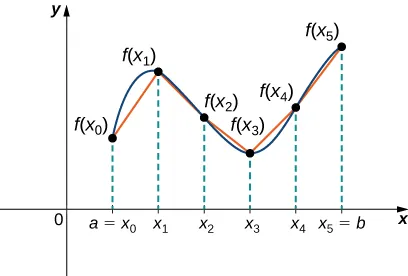
\includegraphics[scale=0.5]{./figures/ezgif.com-webp-to-png (1).png}
    \end{center}
    \end{minipage}
    \bigbreak \noindent 
    \begin{minipage}[]{0.47\textwidth}
        To help us find the length of each line segment, we look at the change in vertical distance as well as the change in horizontal distance over each interval. Because we have used a regular partition, the change in horizontal distance over each interval is given by \(\Delta x\). The change in vertical distance varies from interval to interval, though, so we use \(\Delta y_i = f(x_i) - f(x_{i-1})\) to represent the change in vertical distance over the interval \([x_{i-1},x_i]\), as shown in Figure 2.38. Note that some (or all) \(\Delta y_i\) may be negative.
    
    \end{minipage}
    \begin{minipage}[]{0.47\textwidth}
        \begin{center}
            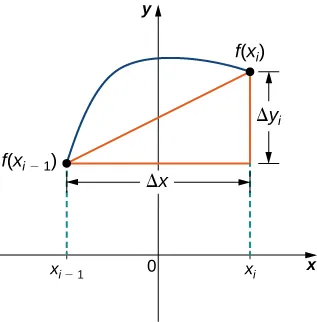
\includegraphics[scale=0.5]{./figures/123.png}
        \end{center}
    
    \end{minipage}

    \pagebreak \bigbreak \noindent 
    By the Pythagorean theorem, the length of the line segment is \(\sqrt{(\Delta x)^2 + (\Delta y_i)^2}\). We can also write this as \(\sqrt{\Delta x^2 + \left(\frac{\Delta y_i}{\Delta x}\right)^2}\).
    \bigbreak \noindent 
    Now, by the Mean Value Theorem, there is a point \(x^*_i \in [x_{i-1},x_i]\) such that \(f'(x^*_i) = \frac{\Delta y_i}{\Delta x}\). Then the length of the line segment is given by \(\sqrt{\Delta x^2 + [f'(x^*_i)]^2}\).
    \bigbreak \noindent 
    Adding up the lengths of all the line segments, we get
    \bigbreak \noindent 
    \[
    \text{Arc Length} \approx \sum_{i=1}^n \sqrt{1 + [f'(x^*_i)]^2}\Delta x.
    \]
    This is a Riemann sum. Taking the limit as \(n \to \infty\), we have
    \[
    \text{Arc Length} = \lim_{n \to \infty} \sum_{i=1}^n \sqrt{1 + [f'(x^*_i)]^2}\Delta x = \int_a^b \sqrt{1 + [f'(x)]^2}\, dx.
    \]
    We summarize these findings in the following theorem.

    \bigbreak \noindent \bigbreak \noindent 
    \begin{thrm}[Arc length for $y=f(x)$]
        Let \(f(x)\) be a smooth function over the interval \([a,b]\). Then the arc length of the portion of the graph of \(f(x)\) from the point \((a,f(a))\) to the point \((b,f(b))\) is given by
        \[
        \text{Arc Length} = \int_a^b \sqrt{1 + [f'(x)]^2} \, dx.
        \]
    \end{thrm}
    \bigbreak \noindent \bigbreak \noindent 
    \nt{Note that we are integrating an expression involving \(f'(x)\), so we need to be sure \(f'(x)\) is integrable. This is why we require \(f(x)\) to be smooth. The following example shows how to apply the theorem.}

    \pagebreak \bigbreak \noindent 
    \begin{eg}[Calculating the Arc Length of a Function of x]
        Let \( f(x) = 2x^{3/2} \). Calculate the arc length of the graph of \( f(x) \) over the interval \([0,1]\). Round the answer to three decimal places.
    \end{eg}
    \bigbreak \noindent 
    \textbf{Solution.} First we find the derivative with respect to $x$:
    \begin{align*}
        \frac{d}{dx}2x^{\frac{3}{2}} =3x^{\frac{1}{2}}
    .\end{align*}
    \bigbreak \noindent 
    By Theorem 12:
    \begin{align*}
        \text{Arc Length} &= \int_{0}^{1}\ \sqrt{1+[3x^{\frac{1}{2}}]^{2}}\ dx \\
          &=\int_{0}^{1}\ \sqrt{1+9x}\ dx 
    .\end{align*}
    \bigbreak \noindent 
    By $u$-sub:
    \bigbreak \noindent 
    \begin{minipage}[]{0.47\textwidth}
        \begin{align*}
            &\text{Let $u=1+9x$} \\
            &du = 9dx \\
            &\frac{1}{9}du = dx  \\
            &u(a) = 1 \quad u(b) = 10
        .\end{align*}
    \end{minipage}
    \begin{minipage}[]{0.47\textwidth}
        Thus:
        \begin{align*}
            &\frac{1}{9}\int_{1}^{10}\ u^{\frac{1}{2}}\ du \\
            &=\frac{2}{27}\left[10^{\frac{3}{2}}-1\right] \\
            &= \frac{2}{27}\left(10\sqrt{10}-1\right)
        .\end{align*}
    \end{minipage}
    \bigbreak \noindent 
    \nt{Although it is nice to have a formula for calculating arc length, this particular theorem can generate expressions that are difficult to integrate. We study some techniques for integration in Introduction to Techniques of Integration. In some cases, we may have to use a computer or calculator to approximate the value of the integral.}
    \bigbreak \noindent 
    \pagebreak 
    \phantomsection
    \addcontentsline{toc}{subsection}{Arc Length of the Curve x = g(y)}
    \subsection*{Arc Length of the Curve x = g(y)}
    \bigbreak \noindent 
    \begin{minipage}[]{0.47\textwidth}
        We have just seen how to approximate the length of a curve with line segments. If we want to find the arc length of the graph of a function of $y$, we can repeat the same process, except we partition the $y$-axis instead of the $x$-axis. Figure 2.39 shows a representative line segment.
    \end{minipage}
    \begin{minipage}[]{0.47\textwidth}
        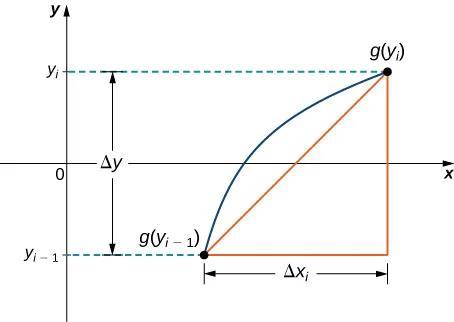
\includegraphics[scale=0.5]{./figures/graph30.png}
    \end{minipage}
    \bigbreak \noindent 
    Then the length of the line segment is $\sqrt{(\Delta y)^2 + (\Delta x_i)^2}$, which can also be written as $\Delta y \sqrt{1 + \left(\frac{\Delta x_i}{\Delta y}\right)^2}$. If we now follow the same development we did earlier, we get a formula for the arc length of a function $x = g(y)$.
    \bigbreak \noindent \bigbreak \noindent 
    \begin{thrm}[Arc Length for $x = g(y)$]
        Let $g(y)$ be a smooth function over a $y$ interval $[c,d]$. Then, the arc length of the graph of $g(y)$ from the point $(g(d), d)$ to the point $(g(c), c)$ is given by
        \[
        \text{Arc Length} = \int_{c}^{d} \sqrt{1 + [g'(y)]^2} \, dy.
        \]
    \end{thrm}

    \pagebreak 
    \phantomsection
    \addcontentsline{toc}{subsection}{Area of a Surface of Revolution}
    \subsection*{Area of a Surface of Revolution}
    \bigbreak \noindent 
    The concepts we used to find the arc length of a curve can be extended to find the surface area of a surface of revolution. Surface area is the total area of the outer layer of an object. For objects such as cubes or bricks, the surface area of the object is the sum of the areas of all of its faces. For curved surfaces, the situation is a little more complex. Let $f(x)$ be a nonnegative smooth function over the interval $[a, b]$. We wish to find the surface area of the surface of revolution created by revolving the graph of $y = f(x)$ around the $x$-axis as shown in the following figure.
    \bigbreak \noindent 
    \begin{center}
        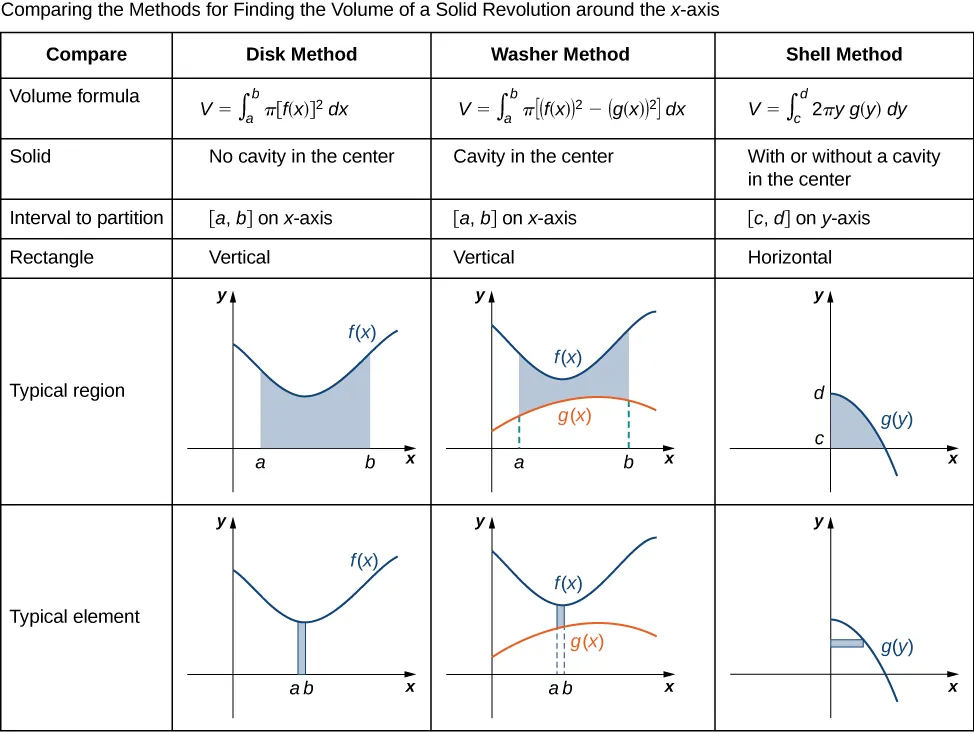
\includegraphics[scale=0.5]{./figures/graph31.png}
    \end{center}
    \bigbreak \noindent 
    As we have done many times before, we are going to partition the interval $[a,b]$ and approximate the surface area by calculating the surface area of simpler shapes. We start by using line segments to approximate the curve, as we did earlier in this section. For $i=0,1,2,\ldots,n$, let $P=\{x_i\}$ be a regular partition of $[a,b]$. Then, for $i=1,2,\ldots,n$, construct a line segment from the point $(x_{i-1},f(x_{i-1}))$ to the point $(x_i,f(x_i))$. Now, revolve these line segments around the $x$-axis to generate an approximation of the surface of revolution as shown in the following figure.
    \bigbreak \noindent 
    \begin{center}
        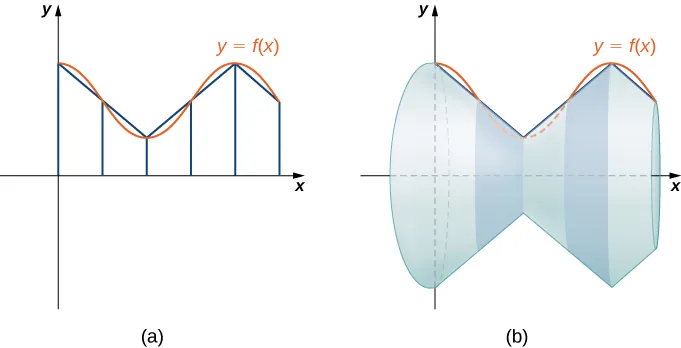
\includegraphics[scale=0.5]{./figures/graph32.png}
    \end{center}

    \pagebreak \bigbreak \noindent 
    Notice that when each line segment is revolved around the axis, it produces a band. These bands are actually pieces of cones (think of an ice cream cone with the pointy end cut off). A piece of a cone like this is called a frustum of a cone.
    \bigbreak \noindent 
    \begin{minipage}[]{0.47\textwidth}
        To find the surface area of the band, we need to find the lateral surface area, $S$, of the frustum (the area of just the slanted outside surface of the frustum, not including the areas of the top or bottom faces). Let $r_1$ and $r_2$ be the radii of the wide end and the narrow end of the frustum, respectively, and let $l$ be the slant height of the frustum as shown in the following figure.
    \end{minipage}
    \begin{minipage}[]{0.47\textwidth}
        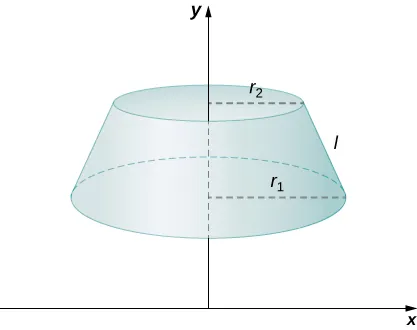
\includegraphics[scale=0.5]{./figures/graph33.png}
    \end{minipage}
    \bigbreak \noindent 
    \begin{minipage}[]{0.47\textwidth}
        We know the lateral surface area of a cone is given by
    \[ \text{Lateral Surface Area} = \pi rs, \]
    where \( r \) is the radius of the base of the cone, and \( s \) is the slant height (see the following figure).
    \end{minipage}
    \begin{minipage}[]{0.42\textwidth}
        \begin{center}
            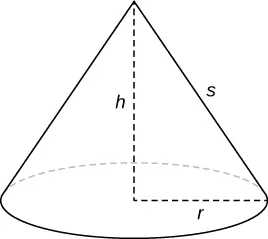
\includegraphics[scale=0.5]{./figures/graph34.png}
        \end{center}
    \end{minipage}
    \bigbreak \noindent 
    \begin{minipage}[]{0.47\textwidth}
        Since a frustum can be thought of as a piece of a cone, the lateral surface area of the frustum is given by the lateral surface area of the whole cone less the lateral surface area of the smaller cone (the pointy tip) that was cut off (see the following figure).
    \end{minipage}
    \begin{minipage}[]{0.49\textwidth}
        \begin{center}
            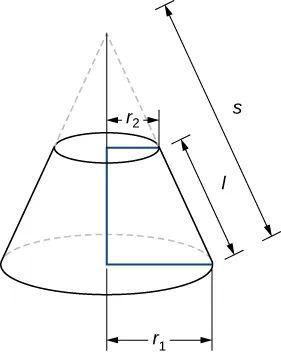
\includegraphics[scale=0.5]{./figures/graph35.png}
        \end{center}
    \end{minipage}
    \bigbreak \noindent 
    \pagebreak \bigbreak \noindent 
    The cross-sections of the small cone and the large cone are similar triangles, so we see that
    \[
    \frac{r_2}{r_1} = \frac{s - l}{s}.
    \]
    Solving for \( s \), we get
    \begin{align*}
        \frac{r_{2}}{r_{1}} &= \frac{s-l}{s} \\
        r_{2}s &= r_{1}(s-l) \\
        r_{2}s &= r_{1}s - r_{1}l \\
        r_{1}l &= r_{1}s - r_{2}s \\
        r_{1}l &= (r_{1} - r_{2})s \\
        s &= \frac{r_{1}l}{r_{1}-r_{2}}
    .\end{align*}
    \bigbreak \noindent 
    Then the lateral surface area (SA) of the frustum is
    \begin{align*}
        &S = (Lateral\ SA\ of\ large\ cone) - (Lateral \, SA \, of \, small \, cone)  \\
        &= \pi r_1 s - \pi r_2 (s - l)  \\
        &= \pi r_1 (r_1 l - r_2) - \pi r_2 (r_1 l - r_2 - l)  \\
        &= \pi r_1^2 l r_1 - r_2 - \pi r_1 r_2 l r_1 - r_2 + \pi r_2 l  \\
        &= \pi r_1^2 l r_1 - r_2 - \pi r_1 r_2 l r_1 - r_2 + \pi r_1 r_2 l r_1 - r_2 - \pi r_2^2 l r_1 - r_2  \\
        &= \pi (r_1^2 - r_2^2) l r_1 - r_2  \\
        &= \pi (r_1 - r_2)(r_1 + r_2) l r_1 - r_2  \\
        &= \pi (r_1 + r_2) l. \\
    .\end{align*}
    \bigbreak \noindent 
    \begin{minipage}[]{0.47\textwidth}
        Let’s now use this formula to calculate the surface area of each of the bands formed by revolving the line segments around the  x-axis. A representative band is shown in the following figure.
    \end{minipage}
    \begin{minipage}[]{0.47\textwidth}
        \begin{center}
            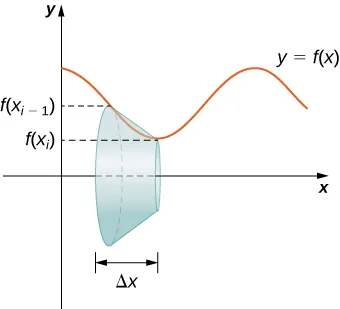
\includegraphics[scale=0.5]{./figures/graph36.png}
        \end{center}
    \end{minipage}

    \pagebreak \bigbreak \noindent 
    Note that the slant height of this frustum is just the length of the line segment used to generate it. So, applying the surface area formula, we have
    \begin{align*}
        &S = \pi(r_1 + r_2)l  \\
        &= \pi\left(f(x_{i-1}) + f(x_i)\right)\sqrt{\Delta x^2 + (\Delta y_i)^2}  \\
        &= \pi\left(f(x_{i-1}) + f(x_i)\right)\sqrt{1 + \left(\frac{\Delta y_i}{\Delta x}\right)^2}. \\
    .\end{align*}
        Now, as we did in the development of the arc length formula, we apply the Mean Value Theorem to select \(x^*_i \in [x_{i-1}, x_i]\) such that \(f'(x^*_i) = \frac{\Delta y_i}{\Delta x}\). This gives us
        \begin{align*}
            S = \pi\left(f(x_{i-1}) + f(x_i)\right)\sqrt{1 + \left(f'(x^*_i)\right)^2}.
        .\end{align*}
        Furthermore, since \(f(x)\) is continuous, by the Intermediate Value Theorem, there is a point \(x^{**}_i \in [x_{i-1}, x_i]\) such that \(f(x^{**}_i) = \frac{1}{2}\left[f(x_{i-1}) + f(x_i)\right]\), so we get
        \begin{align*}
            S = 2\pi f(x^{**}_i)\sqrt{1 + \left(f'(x^*_i)\right)^2}.
        .\end{align*}
        Then the approximate surface area of the whole surface of revolution is given by
        \begin{align*}
            \text{Surface Area} \approx \sum_{i=1}^{n} 2\pi f(x^{**}_i)\sqrt{1 + \left(f'(x^*_i)\right)^2}.
        .\end{align*}
        This almost looks like a Riemann sum, except we have functions evaluated at two different points, \(x^*_i\) and \(x^{**}_i\), over the interval \([x_{i-1}, x_i]\). Although we do not examine the details here, it turns out that because \(f(x)\) is smooth, if we let \(n \to \infty\), the limit works the same as a Riemann sum even with the two different evaluation points. This makes sense intuitively. Both \(x^*_i\) and \(x^{**}_i\) are in the interval \([x_{i-1}, x_i]\), so it makes sense that as \(n \to \infty\), both \(x^*_i\) and \(x^{**}_i\) approach \(x\). Those of you who are interested in the details should consult an advanced calculus text.
        \bigbreak \noindent 
        Taking the limit as \(n \to \infty\), we get
        \begin{align*}
            \text{Surface Area} &= \lim_{{n \to \infty}} \sum_{i=1}^{n} 2\pi f(x^{**}_i)\sqrt{1 + \left(f'(x^*_i)\right)^2}  \\
            &= \int_{a}^{b} \left(2\pi f(x)\sqrt{1 + \left(f'(x)\right)^2}\right) \, dx.
        .\end{align*}
        As with arc length, we can conduct a similar development for functions of \(y\) to get a formula for the surface area of surfaces of revolution about the \(y\)-axis. These findings are summarized in the following theorem.
        \bigbreak \noindent 
        \begin{thrm}[Surface Area of a Surface of Revolution]
           Let \( f(x) \) be a nonnegative smooth function over the interval \([a,b]\).
Then, the surface area of the surface of revolution formed by revolving the graph of \( f(x) \)
around the x-axis is given by
\[
\text{Surface Area} = \int_{a}^{b} \left( 2\pi f(x) \sqrt{1 + \left( f'(x) \right)^2} \right) \, dx.
\]
Similarly, let \( g(y) \) be a nonnegative smooth function over the interval \([c,d]\).
Then, the surface area of the surface of revolution formed by revolving the graph of \( g(y) \)
around the y-axis is given by
\[
\text{Surface Area} = \int_{c}^{d} \left( 2\pi g(y) \sqrt{1 + \left( g'(y) \right)^2} \right) \, dy.
\] 
        \end{thrm}

        \pagebreak 
        \phantomsection
        \addcontentsline{toc}{section}{2.7 Integrals, Exponential Functions, and Logarithms}
        \section*{2.7 Integrals, Exponential Functions, and Logarithms}
        \bigbreak \noindent 

        \phantomsection
        \addcontentsline{toc}{subsection}{The Natural Logarithm as an Integral}
        \subsection*{The Natural Logarithm as an Integral}
        \bigbreak \noindent 
        \smallbreak \noindent
        \begin{definition}
            For $x > 0$, define the natural logarithm function by
            \[
            \ln x = \int_1^x \frac{1}{t} \, dt.
            \]
        \end{definition}
        \bigbreak \noindent 
        \begin{minipage}[]{0.47\textwidth}
        
        For $x > 1$, this is just the area under the curve $y = \frac{1}{t}$ from $1$ to $x$. 
        \bigbreak \noindent 
        For $x < 1$, we have
        \bigbreak \noindent 
        \[
        \int_1^x \frac{1}{t} \, dt = -\int_x^1 \frac{1}{t} \, dt,
        \]
        \bigbreak \noindent 
        so in this case it is the negative of the area under the curve from $x$ to $1$ (see the following figure).
        \end{minipage}
        \begin{minipage}[]{0.47\textwidth}
            \begin{center}
                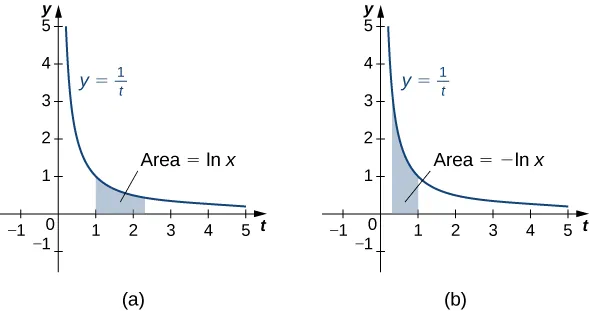
\includegraphics[scale=0.45]{./figures/graph50.png}
            \end{center}
        \end{minipage}
        \bigbreak \noindent 
        Notice that $\ln 1 = 0$. Furthermore, the function $y = \frac{1}{t} > 0$ for $x > 0$. Therefore, by the properties of integrals, it is clear that $\ln x$ is increasing for $x > 0$.

        \bigbreak \noindent 
        \begin{center}
            \begin{Huge}
                \textbf{Section is trivial}
            \end{Huge}
        \end{center}




        








    


    
    

    

  

  
  
  
  






    


    

\end{document}
